\section{SATD削除時のソースコードへの影響についての調査\cite{satd-real-removal}}
\subsection{概要}
文献\cite{satd-removal}では,SATDの削除について主に定量的な観点をもとに調査を行っているが,削除の手法についての詳細な調査は行われていなかった.SATDの削除の手法の調査を行うことで,特定の種類のSATDに対応するためのパターン学習や,それに基づいて開発者への開発手法の提供を行うことが可能になる.
文献\cite{satd-real-removal}では,\cite{satd-removal}をもとに,5つのオープンソースプロジェクトにおいてSATDがどのように削除されているかについての詳細を,以下の3つのRQに基づいて調査している.

\begin{itemize}
  \item RQ 1: SATDが削除された際の手法(クラス削除,メソッド削除など)はどのように分類されるか?
  \item RQ 2: SATDの削除はコミットメッセージに反映されているか?
  \item RQ 3: SATDを削除した際にコードにどのような変更が行われているか?
\end{itemize}

% ====== 結果いるのかな? ==========
% その結果,SATDの削除のうち「偶発的な削除(SATDの削除を目的とせずに行なった開発の中での削除)」は非常に頻繁に(最大50\%の事例)発生しておりで発生しており,実際にコミットメッセージに記録されているSATD削除の割合はかなり限られている(8\%)ことが示されている.SATDがどのように削除されるかについては,ほとんどのケースで複雑な変更が行われていることがわかり,SATDが削除されるパターンとしては,メソッド呼び出しや条件式の変更が繰り返し行われているということが明らかになっている.

\subsection{データの前処理}
文献\cite{satd-real-removal}では,文献\cite{satd-removal}で用いられてるデータを利用し,調査を行っている.

\begin{table}[t]
    \centering
    \caption{データ詳細}
    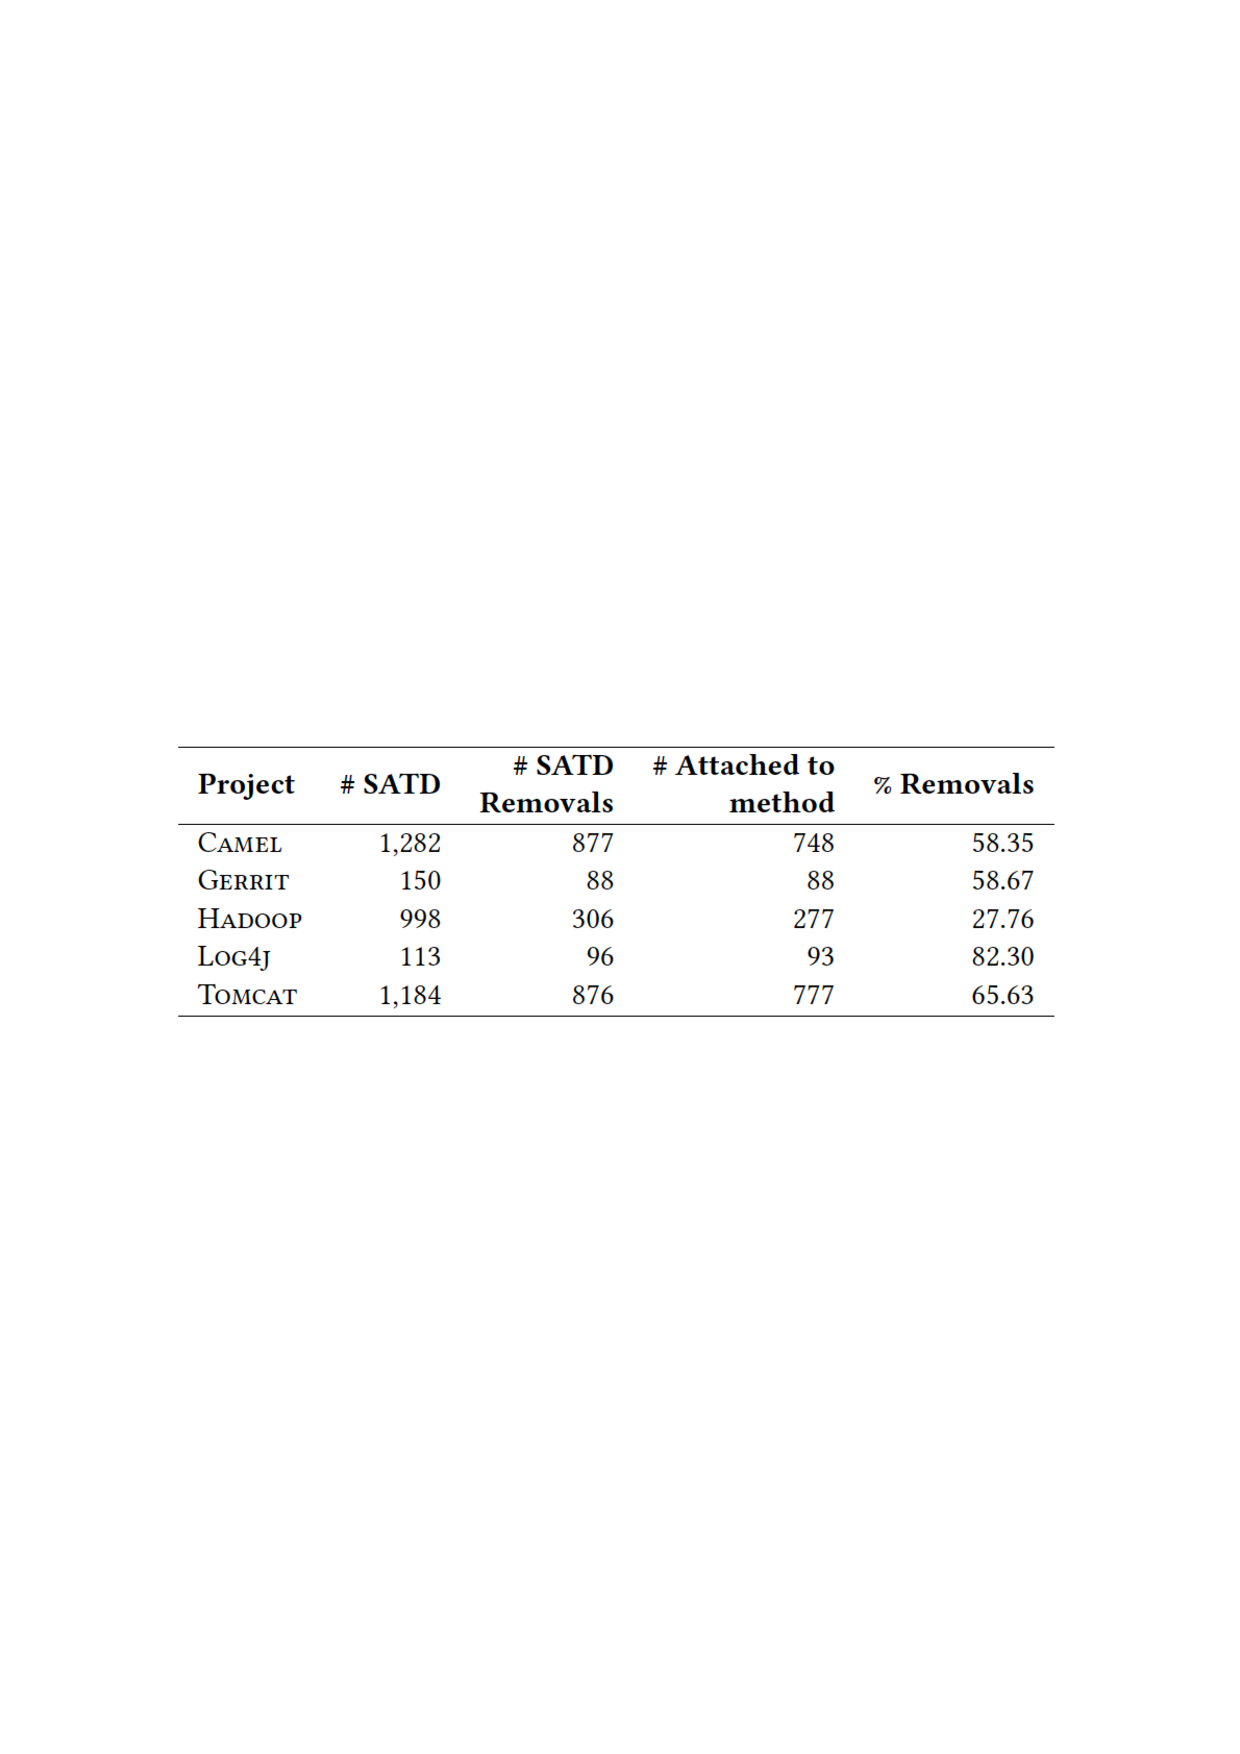
\includegraphics[width=0.9\linewidth, angle=0]{./thesis2/satd-attached-methods2.pdf}
    \label{fig:2_satd-attached-methods}
\end{table}

表\ref{fig:2_satd-attached-methods}にデータの詳細を示す.表\ref{fig:2_satd-attached-methods}では,SATDの重複や不整合を除外したため文献\cite{satd-removal}より総数が少なくなっている.

% ここらへんあんまりわかっていない
また,SATD削除の際のソースコードの変更に着目した調査を行うため,ファイルやクラス全体のSATDは無視して、メソッドレベルのSATDに着目している.
% SATDがメソッド本体に含まれていたり、メソッド定義の直前にコメントが付いていたりする場合は,SATDがメソッドに付いているとみなしている.
その後,SATDの削除として不適切な例として,(1)SATDを含むファイル名の変更が削除と判定されている場合, (2)SATDがコード内の別の場所に移動されている場合,(3)SATDが構文的に変更されたが変更後もSATDを表している場合の3パターンを除外し,表\ref{fig:2_satd-failer-alarm}にその結果を示す.

\begin{table}[t]
    \centering
    \caption{SATD 削除フィルタリング結果}
    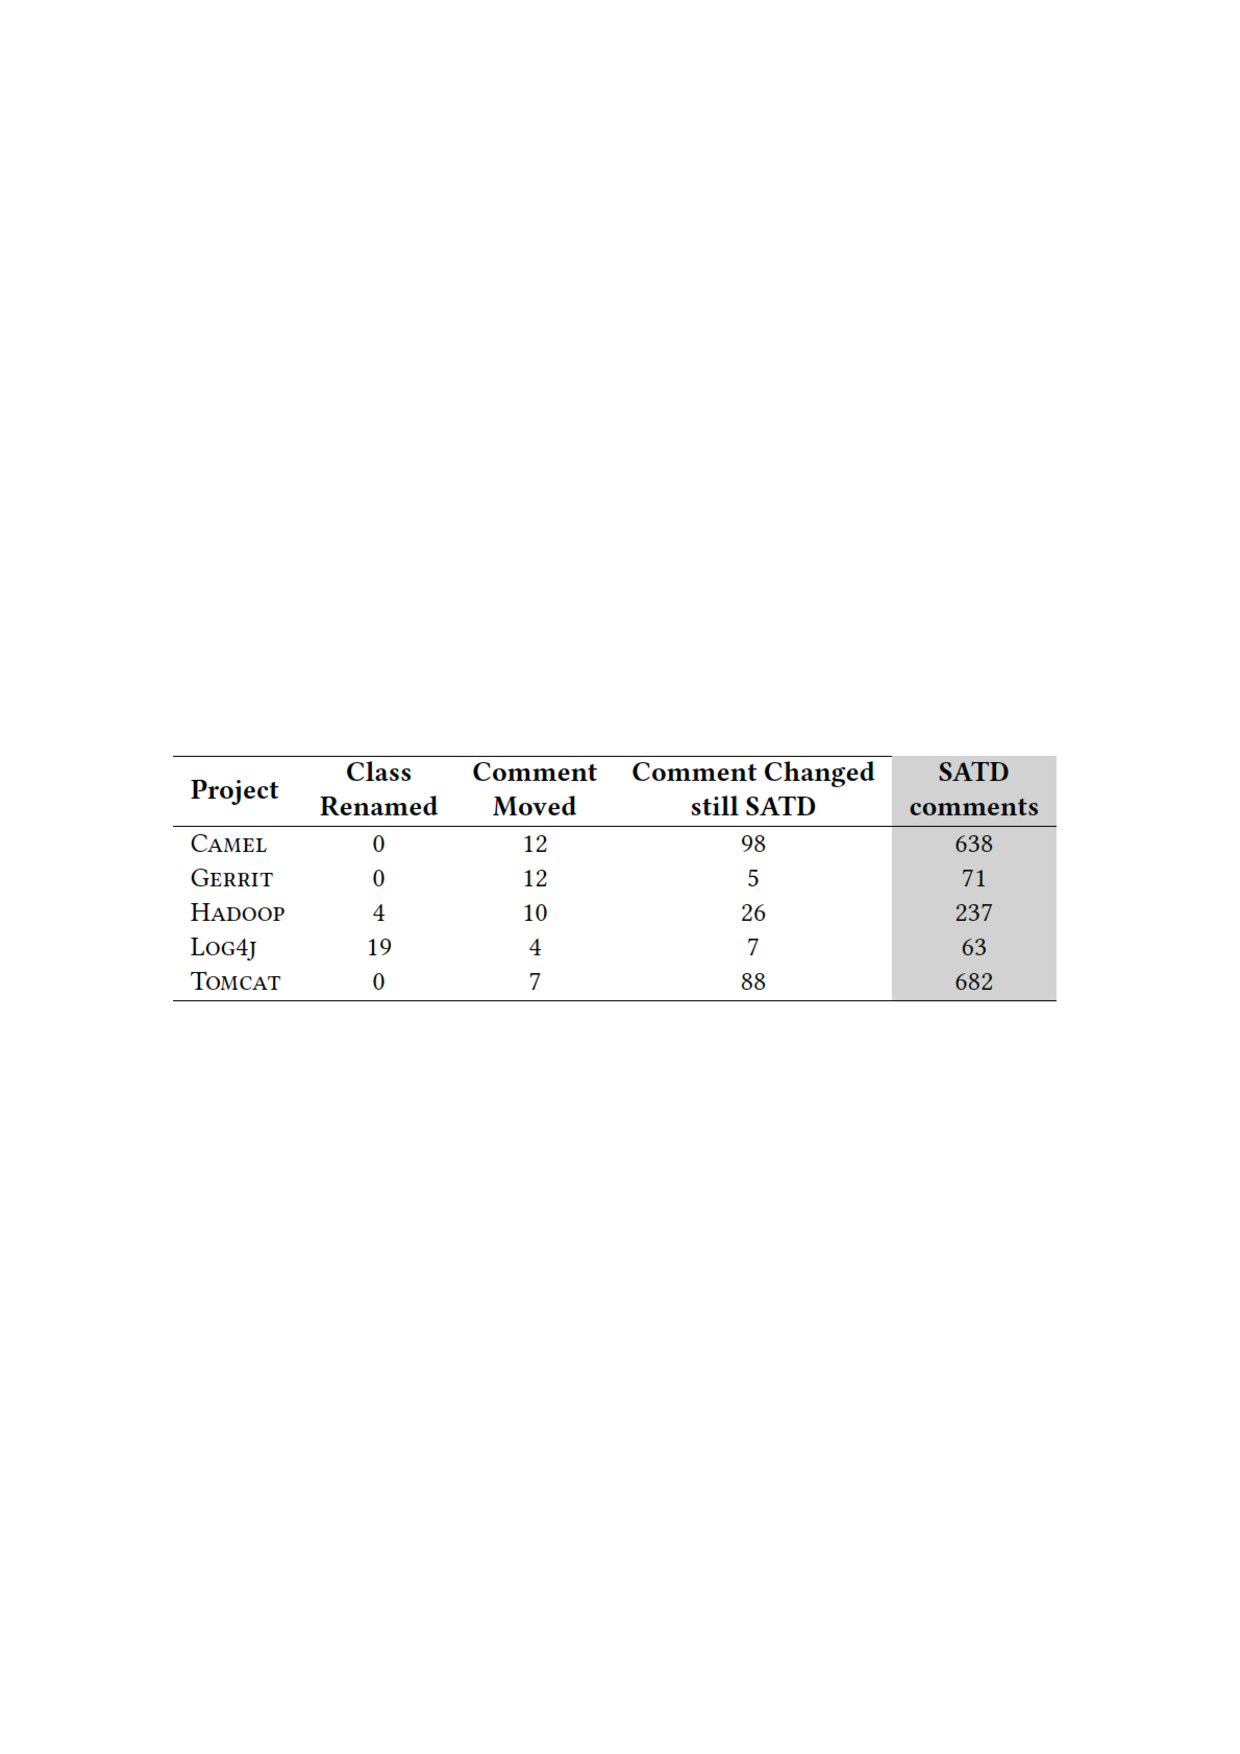
\includegraphics[width=0.9\linewidth, angle=0]{./thesis2/satd-failer-alarm2.pdf}
    \label{fig:2_satd-failer-alarm}
\end{table}

次にコミットメッセージについて,コミットメッセージがSATDの削除について言及しているかどうか判断するために,コミットメッセージと削除されたSATDとのテキストでの類似性をコサイン類似度を用いて分析し,類似している場合を手動で5段階に分類している.

\subsection{結果}
文献\cite{satd-real-removal}では,SATDの削除とソースコードの変更との関係をより深く調査している.その結果,SATDの削除はクラス全体またはメソッド全体が削除された場合に 「偶発的(SATDの削除を目的とせず)」に発生していることが明らかになっている.さらに,SATDの削除がコミットメッセージに明言されているケースは,わずか8\%であり,SATDがどのように削除されるかについては,開発者は複雑な変更を行うだけでなく,メソッドの呼び出しや条件式を変更する傾向があるということが報告されている.

文献\cite{satd-real-removal}では,これらの知見を利用して,SATD埋め込み時のの推奨事項の提供や,ボットへの組み込みを通して,SATDを解決するための提案を提供することができると示唆されている.

DockerにおいてもSATDの管理,解決のために,このような推奨事項の提供やボットの開発は有効であると考えられるため,調査を行うべきである.
